\documentclass[a4paper,12pt]{article}
 \usepackage{graphicx}
 \usepackage{fancyhdr}
 \usepackage{url}
 \usepackage{subfigure}
 \usepackage{geometry}
 \usepackage{caption}
 \usepackage{multirow}
\usepackage{amsmath,amssymb}
\usepackage{CJK}
\usepackage{diagbox}
\usepackage{graphicx}
\usepackage{geometry}
\usepackage{amsfonts}
\usepackage{indentfirst}
%\usepackage{type1cm}
\usepackage{bm}
\usepackage{amsmath}
\usepackage{amssymb}
%\usepackage{minted} %sao
%\usepackage{algorithm} %format of the algorithm %sao
%\usepackage{algorithmic} %format of the algorithm %sao
%\usepackage[ruled]{algorithm2e}%sao
%\usepackage{tcolorbox}%sao
\usepackage{multirow} %multirow for format of table
%\usepackage{xcolor}
\usepackage{color}
%\usepackage{epstopdf}
\usepackage{enumerate}
\usepackage{graphicx}
\usepackage{subfigure}
\usepackage{float}





\usepackage[margin=2cm]{geometry}
\usepackage[utf8]{inputenc}
\usepackage[T1]{fontenc}
\usepackage{lmodern}

\usepackage{mmacells}


\mmaDefineMathReplacement[≤]{<=}{\leq}
\mmaDefineMathReplacement[≥]{>=}{\geq}
\mmaDefineMathReplacement[≠]{!=}{\neq}
\mmaDefineMathReplacement[→]{->}{\to}[2]
\mmaDefineMathReplacement[⧴]{:>}{:\hspace{-.2em}\to}[2]
\mmaDefineMathReplacement{∉}{\notin}
\mmaDefineMathReplacement{∞}{\infty}
\mmaDefineMathReplacement{��}{\mathbbm{d}}


\mmaSet{
  morefv={gobble=2},
  linklocaluri=mma/symbol/definition:#1,
  morecellgraphics={yoffset=1.9ex}
}







\pagestyle{fancy}
 \title{
\includegraphics[scale=1.44]{biaoti.PNG}\\
\vspace{0.3cm} \hrule
\vspace{2.3cm}\huge{{\bf VE401 Term Project 2}}\\ \vspace{1.2cm} \huge{Fatal Traffic Accidents in Shanghai:\\ a predictable pattern?}\vspace{1.2cm}}













\author{
\begin{tabular}{ll}
Hu Zhengdong & 517370910249\\
Wang Yisen & 517370910202\\
Xu Mengjing &517370910042\\
Zhang Hexin & 517370910134\\
Zou Jiayun & 517370910191\\\\\\\\\\
\end{tabular}}

\begin{document}
 	\maketitle
 	\newpage
\section*{Abstract}
\noindent 
\noindent This project mainly analyzes the pattern of fatal traffic accidents in Shanghai from July 1$^{\text{st}}$, 2014 to April 30$^{\text{th}}$, 2015. Firstly, a goodness-of-fit test [1] is performed to test whether the occurrence of fatal traffic accidents follows a Poisson distribution. Next, three multinomial [1] tests are performed to test the dependence of occurrence of fatal traffic accidents on weekdays, districts, and time (hours). Then, using the parameter $k$ of the Poisson distribution, a confidence interval of the occurrence of fatal traffic accidents is derived. Finally, we calculate the prediction interval for the occurrence of fatal traffic accidents. Plus, we also plot the prediction interval, the real data, and estimation of occurrence of fatal traffic accidents to intuitively show the goodness of out test.
	
\newpage\tableofcontents\newpage
\section{Introduction}
\noindent With the development of science and technology, more and more people fint it hard to avoid travelling by automobiles everyday. Nevertheless, significant amounts of people are killed by traffic accidents everyday. Therefore, some questions are raised: is the occurrence of accidents increasing? How to do our best to prevent traffic accidents? [6] As a result, it is urgent for us to study the pattern of traffic accidents. \\\\
In this project, we will mainly study the traffic accidents in Shanghai from July 1$^{\text{st}}$, 2014 to April 30$^{\text{th}}$, 2015. The data are taken from {\emph {SODA}}. [5] Figure 1 shows the number of fatal traffic accidents in Shanghai between July 1$^{\text{st}}$, 2014 and April 30$^{\text{th}}$, 2015.\\ 
\begin{figure}[hbp]
\centering
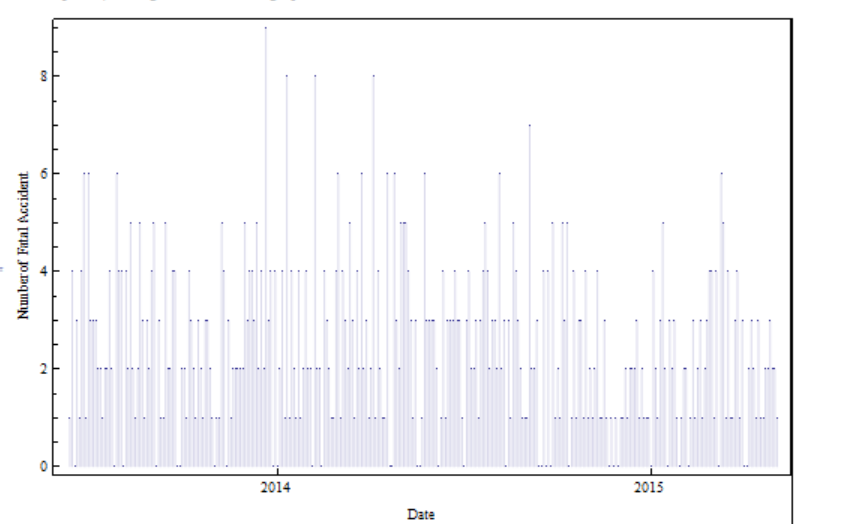
\includegraphics[scale=1]{zongtu.PNG}
\caption{Number of fatal traffic accidents in Shanghai between July 1$^{\text{st}}$, 2014 and April 30$^{\text{th}}$, 2015.}
\end{figure}
\\We would like to provide a brief introduction on our analysis method in the first place.
\subsection{Goodness-of-fit test}
\noindent First, we will use a goodness-of-fit test [1]  to examine whether the occurrence of fatal traffic accidents follows a Poisson distribution. If the follows a Poisson distribution, then the occurrence of traffic accidents in Shanghai is relatively steady; otherwise, the occurrence will not be steady.
\subsection{Confidence interval for parameter $k$}
\noindent Second, we will calculate a confidence interval for the $k$ value of the Poisson distribution. The calculation is based on the assumption that the estimator for k follows a normal distribution on the condition of a large sample size.
\subsection{Dependence of fatal traffic accidents}
\noindent Third, three multinomial [1] tests will be performed to test the dependence of occurrence of fatal traffic accidents on weekdays, districts, and time (hours). The dependence of traffic accidents should be able to determine the distribution of police in Shanghai to some extent. If a certain area or time tends to have more traffic accidents, more police should be attributed to this certain area or time.
\subsection{Prediction interval}
\noindent Finally, we will calculate the prediction interval. We will predict the interval in which the number of future fatal traffic accidents will lie in. The derivation of the prediction interval is based on Nelson's formula [4]. We will first deduce Nelson's formula and then apply this formula to calculate the prediction interval.
\section{Acknowledgement}
\noindent The theme and analysis methods are similar to "London murders: a predictable pattern?" [7] by D. Spiegelhalter and A. Barnett. Our project is based on the selections  and extensions of Spiegelhalter and Barnett's methods. Therefore, we appreciate the efforts done by  Spiegelhalter and Barnett's.
 \section{Goodness of Fit Test}
\noindent To investigate whether the number of traffic fatal accidents follows a Poisson distribution, we apply the goodness-of-fit test to a Poisson distribution with unknown parameter $k$ [1]. The collected data are shown in Table 1.
\newpage
\begin{table}[hbp]
\centering
\begin{tabular}{|c|c|}
\hline
Number of fatal accidents X&Observed days $O_i$\\
\hline
0	&34\\
\hline
1	&71\\
\hline
2	&67\\
\hline
3	&56\\
\hline
4	&43\\
\hline
5	&18\\
\hline
6	&10\\
\hline
7	&1\\
\hline
8	&3\\
\hline
9	&1\\
\hline
\end{tabular}
\caption{Observed number of days with different number of fatal accidents registered by police between  July 1$^{\text{st}}$, 2014 and April 30$^{\text{th}}$, 2015. in Shanghai}
\end{table}

\noindent We know that a maximum-likelihood estimator for $k$ is the sample mean.
\begin{equation}
\widehat{k}=\overline{X}=\frac{1}{304}(34\times 0+71\times 1+67\times 2+56\times 3+43\times 4 
+18\times 5+10\times 6+1\times 7+3\times 8+9\times 1)
\end{equation}
Then we have
\begin{equation}\label{*}
\widehat{k}=2.4178
\end{equation}
\noindent Next, we calculate the probabilities for different categories.
\begin{equation}
\centering
\begin{split}
P[X=0]&=\frac{e^{-\widehat{k}}\widehat{k}^0}{0!}=0.0891\\
P[X=1]&=\frac{e^{-\widehat{k}}\widehat{k}^1}{1!}=0.2155\\
P[X=2]&=\frac{e^{-\widehat{k}}\widehat{k}^2}{2!}=0.2605\\
P[X=3]&=\frac{e^{-\widehat{k}}\widehat{k}^3}{3!}=0.2099\\
P[X=4]&=\frac{e^{-\widehat{k}}\widehat{k}^4}{4!}=0.1269\\
P[X=5]&=\frac{e^{-\widehat{k}}\widehat{k}^5}{5!}=0.0614\\
P[X=6]&=\frac{e^{-\widehat{k}}\widehat{k}^6}{6!}=0.0247\\
P[X=7]&=\frac{e^{-\widehat{k}}\widehat{k}^7}{7!}=0.0085\\
P[X=8]&=\frac{e^{-\widehat{k}}\widehat{k}^8}{8!}=0.0026\\
P[X=9]&=1-P[X=0]-P[X=1]-P[X=2]-P[X=3]-P[X=4]\\
	  &\quad-P[X=5]-P[X=6]-P[X=7]-P[X=8]\\
	  &=0.0009
\end{split}
\end{equation}

\noindent Thus we get the multinomial distribution with parameters $$(p_0,p_1,p_2,p_3,p_4,p_5,p_6,p_7,p_8,p_9)=$$
$$( 0.0891,0.2155,0.2605,0.2099,0.1269,0.0614,0.0247,0.0085,0.0026,0.0007)
$$
\newpage
\noindent We can therefore calculate expected number of days $E_i=np_i$. The results are shown in Table 2.
\begin{table}[hbp]
\centering
\begin{tabular}{|c|c|c|}
\hline
Number of fatal accidents X&Observed days $O_i$&Expected days $E_i$\\
\hline
0&34&27.1\\
\hline
1&71&65.5\\
\hline
2&67&79.2\\
\hline
3&56&63.8\\
\hline
4&43&38.6\\
\hline
5&18&18.7\\
\hline
6&10&7.5\\
\hline
7&1&2.6\\
\hline
8&3&0.8\\
\hline
9&1&0.3\\
\hline
\end{tabular}
\caption{Observed and expected number of days with fatal traffic accidents}
\end{table}

\noindent However, we can see that $E_7$,$E_8$ and $E_9$ are less than 5, which violates the requirement of the Pearson statistic: $E[X_i]=np_i\geq 5$ for $80\%$ of all $i$ [1]. So, we will combine the last three categories. Table 3 shows the result after the change.\\
\begin{table}[hbp]
\centering
\begin{tabular}{|c|c|c|}
\hline
Number of fatal accidents X&Observed days $O_i$&Expected days $E_i$\\
\hline
0&34&27.1\\
\hline
1&71&65.5\\
\hline
2&67&79.2\\
\hline
3&56&63.8\\
\hline
4&43&38.6\\
\hline
5&18&18.7\\
\hline
6&10&7.5\\
\hline
$\ge7$&5&3.7\\
\hline
\end{tabular}
\caption{Observed and expected number of days with fatal traffic accidents}
\end{table}



\newpage
\noindent The plot of observed days and expected days are shown in Figure 2 and Figure 3.
\begin{figure}[hbp]
\centering
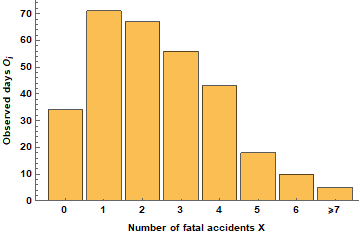
\includegraphics[scale=0.8]{1_11.png}
\caption{Observed days with fatal accidents}
\end{figure}

\begin{figure}[hbp]
\centering
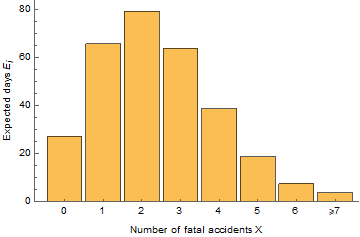
\includegraphics[scale=0.8]{1_21.png}
\caption{Expected days with fatal accidents}
\end{figure}

\noindent The test
\begin{center}
$H_0$: the number of fatal traffic accidents in Shanghai between July 1$^{st}$, 2014 and April 30$^{th}$, 2015 follows a Poisson distribution with parameter $k=2.4178$
\end{center}
 \noindent is then equivalent to the test
\begin{center}
$H_0$: the number of fatal traffic accidents in Shanghai between July 1$^{st}$, 2014 and April 30${th}$, 2015 follows a categorical distribution with parameters $$(p_0,p_1,p_2,p_3,p_4,p_5,p_6,p_7,p_8,p_9)=$$ $$(0.0891,0.2155,0.2605,0.2099,0.1269,0.0614,0.0247,0.0085,0.0026,0.0007)$$
\end{center}

\noindent The statistic
\begin{equation}
X^2=\Sigma_{i=1}^N \frac{(O_i-E_i)^2}{E_i}=6.8634
\end{equation}

\noindent then follows a chi-squared distribution with $N-1-m=8-1-1=6$ degree of freedom. We will reject $H_0$ at a significance of $5\%$.
\begin{equation}
X^2=6.8634<\chi^2_{0.05,6}=12.592
\end{equation}

\noindent We therefore can't reject $H_0$ at a significance of $5\%$, so there is evidence that
 the number of fatal traffic accidents in Shanghai between July 1$^{\text{st}}$, 2014 and April 30$^{\text{th}}$, 2015 follows a Poisson distribution with parameter $k=2.4178$. 
 \section{Confidence interval for parameter $k$}
\noindent Let $X_1\cdots X_n$ be a random sample of size $n$ from a Poisson distribution with parameter $k$, then the mean and variance are given by $\mu=k$ and $\sigma^2=k$. Since we have a large sample size, it's safe to assume that $\overline{X}$ (the estimator for $k$, $\overline{X}=\widehat{k}$) follows a normal distribution with  $\mu=k$ and $\sigma^2=k/n$. [1] Thus
\begin{equation}
Z=\frac{\overline{X}-k}{k/\sqrt{n}}
\end{equation}

\noindent follows a standard normal distribution. The $100(1-\alpha)\%$ confidence interval for $k$ is 
\begin{equation}
\widehat{k}\pm z_{\alpha/2}\frac{k}{\sqrt{n}}
\end{equation}

\noindent However, the interval depends on the unknown parameter $ k$, which is what we are trying to estimate. One solution is to replace $k$ by $\widehat{k}$.
\begin{equation}
\widehat{k}\pm z_{\alpha/2}\frac{\widehat{k}}{\sqrt{n}}
\end{equation}

\noindent Although the number $z_{\alpha/2}$ is no longer accurate, the difference between  $z_{\alpha/2}$ and the correct value is negligible because the sample size n is large enough to allow the central limit theorem to hold [1]. Then for $k=2.4178$, $n=304$, a 95$\%$ confidence interval for k is
\begin{equation}
2.4178\pm 1.96\sqrt{2.4178/304}=2.4178\pm 0.1748
\end{equation}
Then the 95$\%$ confidence interval for parameter $k$ is $[2.2430,2.5926]$.
\section{Dependence of fatal accidents}
 \noindent We've shown that there's evidence the occurrence of fetal traffic accidents in Shanghai follows a Poisson distribution from July 1$^{\text{st}}$, 2014 to April 30$^{\text{th}}$, 2015. However, does the occurrence of fetal traffic accidents depend on some other factors? In this section, we will study relation between the occurrence of fatal traffic accidents with three different factors, i.e. weekdays, districts and time(hours).
 \subsection{Relationship with weekdays}
 \noindent  We are interested in whether the probability of accidents to happen on each weekdays is the same. This is because it is reasonable to assume that accidents are easier to happen on Mondays since most people are not in a good mood on Mondays; accidents are less likely to happen at Weekends since their are fewer cars on the road at weekends. Thus, we want to study the relationship the occurrence of fatal traffic accidents with different weekdays.
\\\\Figure 4 shows the relationship between fatal traffic accidents and different weekdays.
\begin{figure}[hbp]
\centering
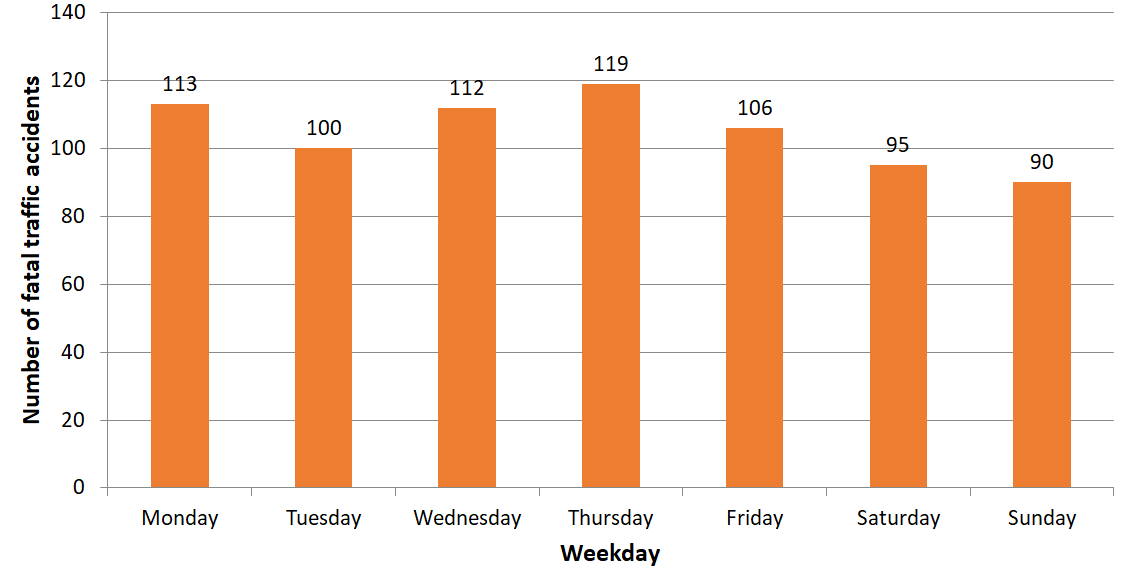
\includegraphics[scale=0.6]{weekday2.PNG}
\caption{Relationship between fatal traffic accidents and  weekdays}
\end{figure}
\noindent\\The total number is $n=735$. We will use a Multinomial Trial [1] to test if the number of fetal traffic accidents depends on weekdays. As a result, we set the null hypothesis to be\\\\
\centerline{$H_0:$ The data follow a multinomial distribution}
\centerline{with parameter $(p_1,...,p_7)=(\frac{1}{7},...,\frac{1}{7})$}
 %\noindent \\\\
 \\\\So the observed value and the expected value can be represented by
 \begin{table}[H]\centering
\begin{tabular}{|c|c|c|c|c|c|c|c|}
\hline
 &Monday&Tuesday&Wednesday&Thursday&Friday&Saturday&Sunday  \\ \hline
$O_i$&113&100&112&119&106&95&90\\ \hline
$E_i$&105&105&105&105&105&105&105\\ \hline
\end{tabular}
\caption{Observed value and the expected value of  weekdays}
\end{table}
\noindent
In which $E_i=np_i=735\cdot 1/7=105$ for $1\leq i\leq 7$ and $n\in\mathbb{N}$. Therefore,
\begin{equation}\label{weekday}
\begin{split}
X_{k-1}^{2}&=\sum_{i=1}^{k} \frac{\left(O_{i}-E_{i}\right)^{2}}{E_{i}}\\
X_{7-1}^{2}&=\sum_{i=1}^{7} \frac{\left(O_{i}-E_{i}\right)^{2}}{E_{i}}\\
&=\frac{(113-105)^{2}}{105}+\frac{(100-105)^{2}}{105}
+\cdots+\frac{(90-105)^{2}}{105}
\\&=6.286
\end{split}
\end{equation}
Checking the chi-square distribution table [3], we can find that $\chi_{0.3,6}^{2}=7.231$, then
$$X_{7-1}^{2}<\chi_{0.3,6}^{2}$$
Namely, we cannot reject $H_0$ at significance level 0.3. In other word, the P-Value of $H_0$ is greater than 30\% (which is really big). Therefore, we do not have evidence that
$$(p_1,...,p_7)\neq(\frac{1}{7},...,\frac{1}{7})$$
As a result, we have no evidence that the probability of fatal accidents  happen on different weekdays are different. Namely, we have no evidence that number of fatal traffic accidents in Shanghai depends on different weekdays.
\subsection{Relationship with districts}
\noindent  We are interested in whether there is a relation between accidents and different districts. Someone may argue that accidents are more likely to happen in rural districts since there are more trucks travelling in rural districts; and trucks are more likely to cause traffic accidents due to the large inertia and week eyesight of the trucks. However, other people may argue that traffic accidents are more likely to happen in downtown districts, simply because there are more cars and population in downtown. Thus, we want to study the relationship between the occurrence of fatal traffic accidents and different districts.
Figure 5 shows the relationship between fatal traffic accidents and different districts.\\
\begin{figure}[hbp]
\centering
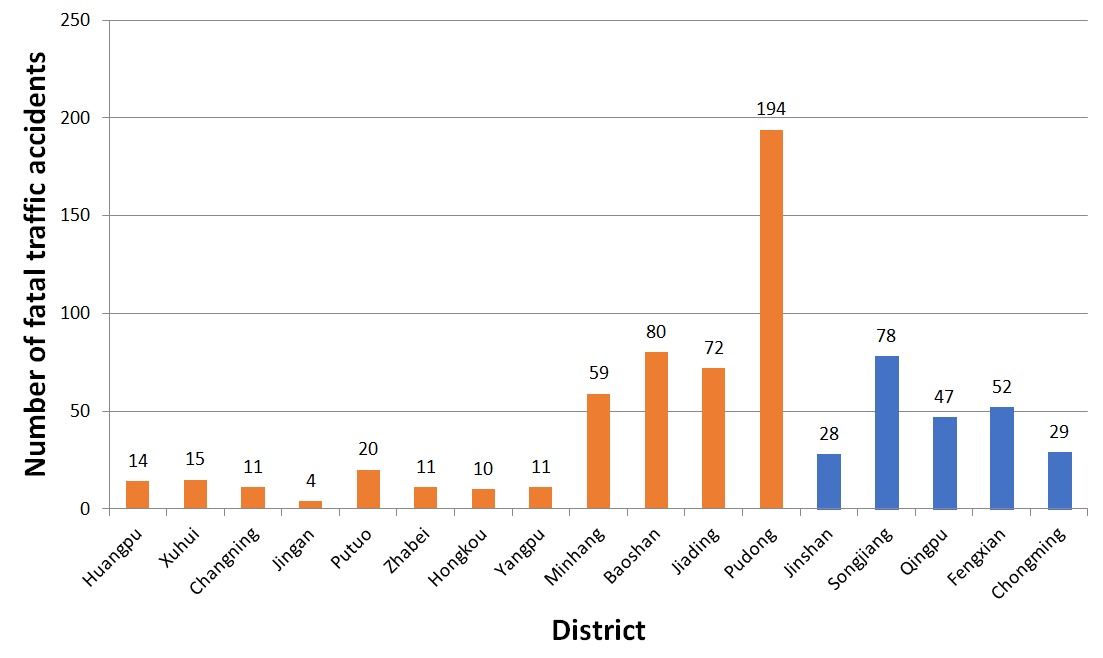
\includegraphics[scale=0.75]{district.PNG}
\caption{Relationship between fatal traffic accidents and  districts\\Orange bar: downtown district$\quad$Blue bar: rural districts [2]}
\end{figure}
\noindent \\The total number is $n=735$. We will use a Multinomial Trial [1] to test if the number of fetal traffic accidents depends on districts. Since the area between different districts are different, although we have 17 districts, the expected probability of each district cannot be 1/17.\\\\
Assume fatal traffic accidents are evenly distributed in all areas in Shanghai, then the expected probability of the $i^{th}$ district should be
\begin{equation}\label{districtP}
p_i=\frac{\text{area of the }i^{th}\text{ district}}{\text{total area of Shanghai}}
\end{equation}
where $1\leq i\leq 17$ and $n\in\mathbb{N}$. Therefore, we calculate the $p_i$ value for each district in the following table by applying eq. \eqref{districtP}.
\begin{table}[H]\centering
\begin{tabular}{|c|c|c|c|c|c|c|}
\hline
&Huangpu&Xuhui&Changning&Jingan&Putuo&Zhabei\\ \hline
Area (km$^2$)&20&55&38&8&55&29\\ \hline
$p_i$&0.0031&0.0087&0.0060&0.0013&0.0087&0.0046\\ \hline\hline
&Hongkou &Yangpu&Minhang&Baoshan&Jiading&Pudong\\ \hline
Area (km$^2$)&23&61&371&271&464&1211\\ \hline
$p_i$&0.0036&0.0096&0.0585&0.0427&0.0732&0.1910\\ \hline\hline
&Jinshan &Songjiang&Qingpu&Fengxian&Chongming&Total\\ \hline
Area (km$^2$)&586&606&670&687&1185&6340\\ \hline
$p_i$&0.0924&0.0956&0.1057&0.1084&0.1869&N/A\\ \hline
\end{tabular}
\caption{Area and $p_i$ value of different districts [2]}
\label{table:area_p}
\end{table}
\noindent Note that the first two rows of table \ref{table:area_p} represent downtown districts and the last row of table \ref{table:area_p} represent rural districts. Then, we can set the null hypothesis to be
\\\\
\centerline{$H_0:$ Fatal traffic accidents are evenly distributed in all areas in Shanghai}
\\\\According to our assumption, as well as 
eq. \eqref{districtP}, this null hypothesis is equivalent to \\\\
\centerline{$H_0:$ The data follow a multinomial distribution}
\centerline{with parameter $(p_1,p_2,...,p_{17})$ from table \ref{table:area_p}}
 %\noindent \\\\
 \\\\So the observed value and the expected value can be represented by
\begin{table}[H]\centering
\begin{tabular}{|c|c|c|c|c|c|c|}
\hline
&Huangpu&Xuhui&Changning&Jingan&Putuo&Zhabei\\ \hline
$O_i$&14&15&11&4&20&11\\ \hline
$E_i$&2.3&6.3&4.4&0.9&6.4&3.4\\ \hline\hline
&Hongkou &Yangpu&Minhang&Baoshan&Jiading&Pudong\\ \hline
$O_i$&10&11&59&80&72&194\\ \hline
$E_i$&2.67&7.07&43.0&31.4&53.8&140.4\\ \hline\hline
&Jinshan &Songjiang&Qingpu&Fengxian&Chongming&Total\\ \hline
$O_i$&28&78&47&52&29&735\\ \hline
$E_i$&67.9&70.3&77.7&79.6&137.4&N/A\\ \hline
\end{tabular}
\caption{Observed value and the expected value of different districts}
\label{table:area_OEii}
\end{table}
\noindent In which $E_i=np_i$ for $1\leq i\leq 17$ and $n\in\mathbb{N}$. Please note that the first two rows of table \ref{table:area_OEii} represent downtown districts and the last row of table \ref{table:area_OEii} represent rural districts. Therefore,
\begin{equation}\label{district}
\begin{split}
X_{k-1}^{2}&=\sum_{i=1}^{k} \frac{\left(O_{i}-E_{i}\right)^{2}}{E_{i}}\\
X_{17-1}^{2}&=\sum_{i=1}^{17} \frac{\left(O_{i}-E_{i}\right)^{2}}{E_{i}}\\
&=\frac{(14-2.3)^{2}}{2.3}+\frac{(15-6.3)^{2}}{6.3}
+\cdots+\frac{(29-137.4)^{2}}{137.4}
\\&=398.62
\end{split}
\end{equation}
Checking the chi-square distribution table [3], we can find that $\chi_{0.005,16}^{2}=34.27$, then
$$X_{17-1}^{2}>\chi_{0.05,23}^{2}$$
Therefore, we have strong evidence to reject $H_0$. Namely, we reject that fatal traffic accidents are evenly distributed in all areas in Shanghai at significance level 0.005.
\\\\Take a deeper look that table at table \ref{table:area_OE}, we find that all the expected values of 15 downtown districts are smaller than the observed values; while almost all the expected values of downtown districts are greater than the observed values  (4 out of 5, except Songjiang District). Therefore, we support the claim that fatal traffic accidents are more likely to happen in downtown districts in Shanghai.\\\\
In short, we have strong evidence that number of fatal traffic accidents in Shanghai depends on different districts.
\subsection{Relationship with time}
\noindent  We are interested in whether there is a relation between accidents and different hour in each day. It is easy to assume that fatal accidents are more likely to happen in the days than at nights. Therefore, we'd like to test if there's a a relation between accidents and different hour in each day.\\\\Figure 6 shows the relationship between fatal traffic accidents and different hours.\\ \newpage
\begin{figure}[hbp]
\centering
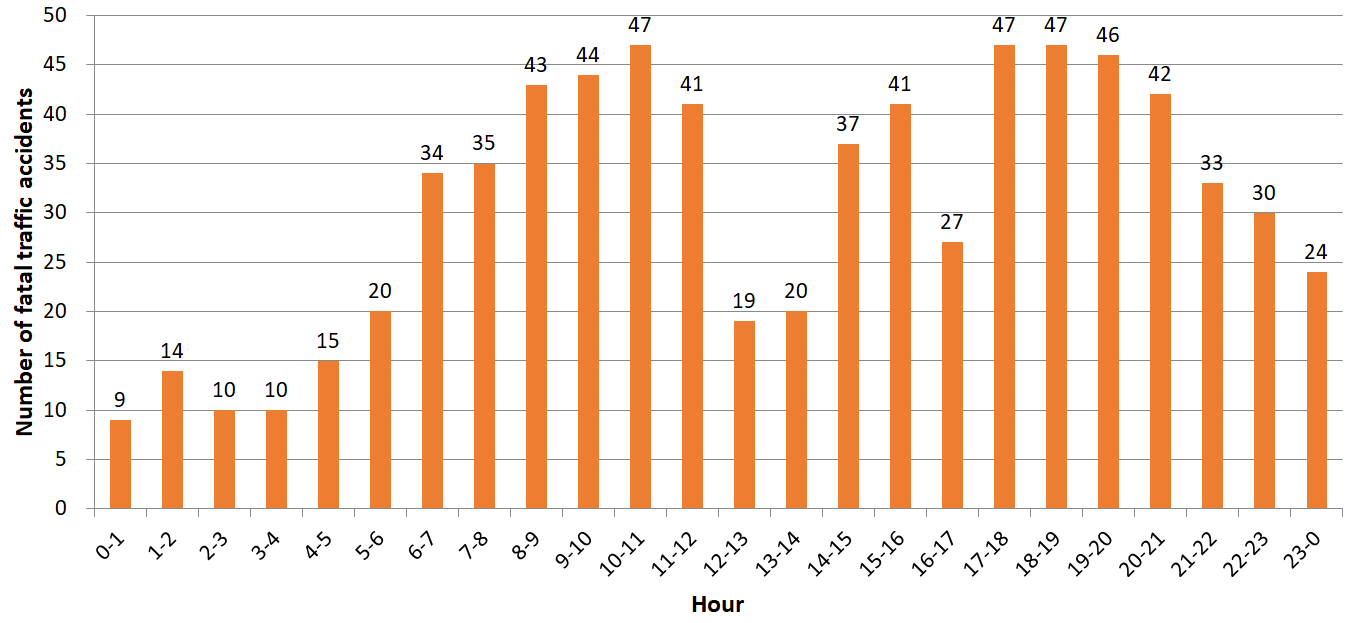
\includegraphics[scale=0.65]{hour.PNG}
\caption{Relationship between fatal traffic accidents and  hours}
\end{figure}
\noindent The total number is $n=735$. We will use a Multinomial Trial [1] to test if the number of fetal traffic accidents depends on hours.
As a result, we set the null hypothesis to be\\\\
\centerline{$H_0:$ The data follow a multinomial distribution}
\centerline{with parameter $(p_1,...,p_{24})=(\frac{1}{24},...,\frac{1}{24})$}
 %\noindent \\\\
 \\\\So the observed value and the expected value can be represented by
\begin{table}[H]\centering
\begin{tabular}{|c|c|c|c|c|c|c|}
\hline
&0:00-0:59&1:00-1:59&2:00-2:59&3:00-3:59&4:00-4:59&5:00-5:59\\ \hline
$O_i$&9&14&10&10&15&20\\ \hline
$E_i$&30.625&30.625&30.625&30.625&30.625&30.625\\ \hline\hline
&6:00-6:59&7:00-7:59&8:00-8:59&9:00-9:59&10:00-10:59&11:00-11:59\\ \hline
$O_i$&34&35&43&44&47&41\\ \hline
$E_i$&30.625&30.625&30.625&30.625&30.625&30.625\\ \hline\hline
&12:00-12:59 &13:00-13:59&14:00-14:59&15:00-15:59&16:00-16:59&17:00-17:59\\ \hline
$O_i$&19&20&37&41&27&47\\ \hline
$E_i$&30.625&30.625&30.625&30.625&30.625&30.625\\ \hline
\hline
&18:00-18:59 &19:00-19:59&20:00-20:59&21:00-21:59&22:00-22:59&23:00-23:59\\ \hline
$O_i$&47&46&42&33&30&24\\ \hline
$E_i$&30.625&30.625&30.625&30.625&30.625&30.625\\ \hline
\end{tabular}
\caption{Observed value and the expected value of  hours}\label{table:area_OE}
\end{table}
\noindent In which $E_i=np_i=73\cdot1/24=30.625$ for $1\leq i\leq 24$ and $n\in\mathbb{N}$. Therefore,
\begin{equation}\label{hourp}
\begin{split}
X_{k-1}^{2}&=\sum_{i=1}^{k} \frac{\left(O_{i}-E_{i}\right)^{2}}{E_{i}}\\
X_{24-1}^{2}&=\sum_{i=1}^{24} \frac{\left(O_{i}-E_{i}\right)^{2}}{E_{i}}\\
&=\frac{(9-30.625)^{2}}{30.625}+\frac{(14-30.625)^{2}}{30.625}
+\cdots+\frac{(24-30.625)^{2}}{30.625}
\\&=132.30
\end{split}
\end{equation}
Checking the chi-square distribution table [3], we can find that $\chi_{0.005,23}^{2}=44.18$, then
$$X_{24-1}^{2}>\chi_{0.005,23}^{2}$$
Therefore, we have strong evidence to reject $H_0$. Namely, we reject that fatal traffic accidents are evenly distributed in all times in Shanghai at significance level 0.005.\\\\
In short, we have strong evidence that number of fatal traffic accidents in Shanghai depends on different hours.

\section{Nelson's Formula and the Prediction Interval}
\noindent We will first derive Nelson's Formula and then apply this formula to calculate the prediction interval of the number of fatal raffic accidents. \\\\
Let us denote the total arrivals in a sample size $n$ from a Poisson distribution as $X$. The mean arrivals of the unit population size is $k$. Let $Y$ be the future total arrivals in a sample size $m$ from the same Poisson distribution. We can derive the expression of $\widehat{k}$, the estimator of $k$.\\
\begin{equation}\label{1}
\widehat{k}=\frac{X}{n}
\end{equation}
$\widehat{k}$ is an unbiased estimator, because
\begin{equation}\label{2}
E[\widehat{k}]=\frac{E[X]}{n}=\frac{nk}{n}=k
\end{equation}
Besides, we can derive the expression of $\widehat{Y}$, the estimator of $Y$ as 
\begin{equation}\label{3}
\widehat{Y}=m\widehat{k}=\frac{mX}{n}
\end{equation}
%$\widehat{Y}$ is also an unbiased estimator, since
The expectation of $\widehat{Y}$ can be calculated as
\begin{equation}\label{4}
E[\widehat{Y}]=\frac{m}{n}E[X]=\frac{m}{n}nk=mk=E[Y]
\end{equation}
and we can conclude that $\widehat{Y}$ is an unbiased estimator of $Y$.\\
Since $X\text{ and }Y$ both follow Poisson distribution, we know that the expectation and variance of $X$ is 
\begin{equation}\label{5}
\begin{aligned}
E[X]&=nk\\
\text{Var} (X)&=nk\\
\end{aligned}
\end{equation}
Similarly, the expectation and variance of $Y$ can be expressed as 
\begin{equation}\label{6}
\begin{aligned}
E[Y]&=mk\\
\text{Var} (Y)&=mk
\end{aligned}
\end{equation}
Therefore, for the variable $\widehat{Y}-Y$, we can calculate its expectation and variance as follows. Note that $X$ and $Y$ are independent, so Cov$(X,Y)=0$.
\begin{equation}\label{7}
\begin{aligned}
E[\widehat{Y}-Y]&=mk-mk=0\\
\text{Var}(\widehat{Y}-Y)&=\text{Var}(\frac{mX}{n}-Y)\\
&=\frac{m^2}{n^2}\text{Var}(X)+\text{Var}(Y)\\
&=\frac{m^2}{n^2}nk+mk\\
&=m^2k(\frac{1}{n}+\frac{1}{m})
\end{aligned}
\end{equation}
Therefore, $\widehat{\text{Var}}(\widehat{Y}-Y)$, the estimator of the variance can be expressed as 
\begin{equation}\label{8}
\widehat{\text{Var}}(\widehat{Y}-Y)=m^2\widehat{k}(\frac{1}{n}+\frac{1}{m})
\end{equation}
By the Central Limit Theorem, we know that 
\begin{equation}\label{9}
\frac{\widehat{Y}-Y}{\widehat{\text{Var}}(\widehat{Y}-Y)}=\frac{\widehat{Y}-Y}{m^2\widehat{k}(\frac{1}{n}+\frac{1}{m})}
\end{equation}
follows a standard normal distribution if sample sizes are large. Therefore, we can derive the $100(1-\alpha$)\% prediction interval. [4]
\begin{equation}\label{10}
\widehat{Y}\pm z_{\alpha/2}\sqrt{m\widehat{Y}(\frac{1}{n}+\frac{1}{m})}
\end{equation}
Eq. \eqref{10} is called the Nelson's prediction interval. When $X=0$, we can calculate that $ \widehat{k}=0,$ so the prediction interval is not defined. Usually we let $\widehat{Y}$ to be $\frac{m}{2n}$ when $X=0$.\\\\
Now we can use Nelson's formula and traffic accident data between July 1$^{st}$, 2014 and April 30$^{th}$, 2015 to derive a prediction interval for fatal traffic accidents in 2019. $\widehat{k}$, the estimator of $k$, is just the mean $\overline{X}$ by the method of maximum likelihood. We know the total sample size is 
\begin{equation*}
n=31+31+30+31+30+31+31+28+31+30=304
\end{equation*}
The total number of fatal traffic accidents in the given sample is 735. Therefore, $\widehat{k}$ can be expressed as 
\begin{equation}\label{11}
\widehat{k}=\frac{735}{304}=2.4178
\end{equation}
We can get the 95\% prediction interval as
\begin{equation}\label{12}
\widehat{Y}\pm 1.96\sqrt{\frac{\widehat{Y}^2}{2.4178}(\frac{2.4178}{\widehat{Y}}+\frac{1}{304})} \text{ or } 2.4178m\pm 1.96\sqrt{2.4178m^2(\frac{1}{m}+\frac{1}{304})}
\end{equation}
Since the number of fatal traffic accidents is discrete, we should modify the prediction interval in Eq. \eqref{12} to be collections of integers within the interval
\begin{equation}\label{13}
\left[ \lceil L \rceil, \lfloor U \rfloor\right]
\end{equation}
Here $\lceil L \rceil$ is the smallest integer greater than or equal to the lower bound of the prediction interval, and $\lfloor U \rfloor$ is the largest integer smaller than or equal to the upper bound of the prediction interval. Figure 7 shows the estimated number of fatal traffic accidents in 2019 and its 95\% prediction interval. We have rounded estimated the number of fatal traffic accidents to the nearest integer. \\
\begin{figure}[!htbp]
\centering
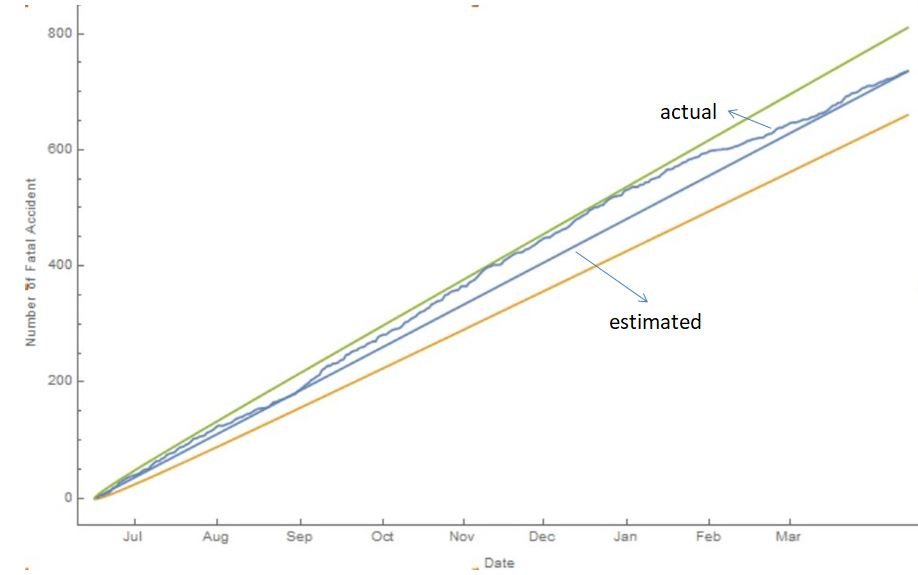
\includegraphics[width=12 cm]{1.jpg}
\caption{Actual and estimated cumulative number of fatal traffic accidents and the prediction interval}
\end{figure}\\
\newpage
\noindent The green line and the orange line are the upper bound and the lower bound of the prediction interval respectively. We are 95\% sure that the true number of fatal traffic accidents in future will fall into the prediction interval. The blue line is the estimation of the cumulative number of fatal traffic accidents, and the curve shows the actual number between July 1$^{st}$, 2014 and April 30$^{th}$, 2015. We can observe that the prediction interval grows wider along $x$-axis. This is because $\widehat{Y}$ is the estimated cumulative number of fatal accidents, and $\widehat{Y}$ becomes bigger as days pass by. The larger $\widehat{Y}$ leads to the wider prediction interval.
\section{Conclusion}
\noindent Through this project, we have analyzed some basic patterns of fatal traffic accidents in Shanghai from July 1$^{\text{st}}$, 2014 to April 30$^{\text{th}}$, 2015. \\\\
In the first place, we perform the goodness-of-fit test, and accept that the null hypothesis that number of fatal traffic accidents in Shanghai from July 1$^{\text{st}}$, 2014 to April 30$^{\text{th}}$, 2015 follows a Poisson distribution with $$k=2.4178$$
 along with a confidence interval of $k$
 $$k\in[2.2430,2.5926]$$
Then, through the mulinomial tests, we find that from July 1$^{\text{st}}$, 2014 to April 30$^{\text{th}}$, 2015:
\begin{enumerate}
    \item We have no evidence that number of fatal traffic accidents in Shanghai depends on different weekdays. 
\item We have strong evidence that number of fatal traffic accidents in Shanghai depends on different districts. Plus,  fatal traffic accidents are more likely to happen in downtown districts in Shanghai than in rural districts.
\item We have strong evidence that number of fatal traffic accidents in Shanghai depends on different hours.
\end{enumerate}

\noindent Last but not least, we calculate the prediction interval based on Nelson's formula. We first provide the derivation of Nelson's formula. We plot the 95\% prediction interval as well as the estimated number of fatal traffic accidents, and we find that the prediction interval is reasonable.

\newpage
\section{Reference}
\noindent [1] Horst Hohberger. Probabilistic Methods in Engineering, University of Michigan \phantom{[1] }- Shanghai Jiaotong University
Joint Institute, Summer Term 2019.\\


\noindent
[2] Askci. The population, area and GDP of every distict in Shanghai in 2015. \phantom{[1] }http://blog.sina.com.cn/s/blog\_14ecaf8630102xes2.html. [Online; accessed July \phantom{[1] }29, 2019].\\

\noindent
[3] Morris H. DeGroot and Mark J. Schervish. Probability and Statistics, Fourth \phantom{[1] }Edition.\\

\noindent[4] K.krishnamoorthy and Jie Peng. "Improved Closed-form Prediction Intervals \phantom{[1] }for Binomial and Poisson Distributions." \emph{Journal of Statistical Planning and \phantom{[1] }Inference}, 141(5): 1709-1718,2011. http://www.sciencedirect.com/science/article\\ \phantom{[1] }/pii/ S0378375810005215.\\

\noindent[5] Shanghai Open Data Applications (SODA). Data provided by the Shanghai \phantom{[1] }Public Security Bureau for the
2019 competition. http://soda.shdataic.org.cn/. \phantom{[1] }[Online; accessed July 11, 2019].\\

\noindent [6] Horst Hohberger. Ve401\_summer2019\_project\_2, University of Michigan - \phantom{[1] }Shanghai Jiaotong University
Joint Institute, Summer Term 2019.\\

\noindent [7] D. Spiegelhalter and A. Barnett. London murders: a predictable pattern? \phantom{[1] }\emph {Significance}, 6(1):5–8, 2009.
http://onlinelibrary.wiley.com/doi/10.1111/j.\\\phantom{[1] }1740-9713.2009.00334.x/abstract.
\newpage
\section{Appendix}
\subsection{Data processing}
\noindent Since we cannot upload the affiliated "Data processing.xlsx", we can only briefly describe our method. We used "filter" to first filter out the death cases from all cases. Then we used "MID", "FIND", "LEFT", modified the output format, and "COUNTIF" to find out the frequencies for different weekdays. With "COUNTIF" and "LEFT", we were able to find out the frequencies for different districts. Similarly, we found out the frequencies for different hours. We found out how many fatal accidents happened everyday and counted the number of days for each fatal accident frequencies.

\subsection{Mathematica code of plotting figure 1}
\begin{mmaCell}[functionlocal=y]{Code}
  ListPlot[{1, 4, 0, 3, 1, 4, 6, 1, 6, 3, 3, 3, 2, 2, 1, 
  2, 2, 4, 2, 0, 6, 4, 4, 0, 4, 2, 5, 2, 1, 2, 5, 3, 1, 
  3, 2, 4, 5, 0, 3, 1, 1, 5, 2, 2, 4, 4, 0, 0, 2, 2, 1, 
  4, 3, 2, 1, 3, 2, 1, 3, 3, 2, 1, 0, 1, 1, 5, 4, 0, 3,
  1, 2, 2, 2, 2, 2, 5, 3, 4, 4, 3, 5, 2, 4, 2, 9, 3, 4,
  0, 4, 0, 2, 4, 1, 8, 1, 4, 2, 1, 4, 1, 2, 4, 2, 2, 0,
  8, 2, 2, 0, 4, 3, 2, 1, 1, 4, 6, 1, 4, 3, 2, 5, 3, 1,
  4, 2, 6, 2, 3, 1, 2, 8, 1, 4, 2, 1, 1, 6, 0, 0,
  6, 3, 2, 5, 5, 5, 4, 3, 1, 3, 0, 0, 1, 6, 3, 3, 3,
  3, 2, 0, 1, 4, 1, 3, 3, 3, 4, 3, 3, 1, 0, 3, 4, 2,
  2, 3, 1, 3, 4, 5, 4, 2, 3, 3, 2, 6, 2, 3, 0, 3, 1,
  5, 4, 3, 2, 1, 1, 1, 7, 2, 2, 3, 0, 0, 4, 0, 4, 0,
  5, 1, 2, 1, 5, 3, 5, 0, 1, 4, 1, 3, 3, 1, 4, 1, 2,
  1, 2, 4, 1, 1, 3, 1, 0, 1, 0, 1, 0, 1, 1, 2, 1, 2,
  2, 2, 3, 1, 2, 1, 1, 1, 0, 4, 2, 1, 3, 5, 2, 0, 3, 
  2, 3, 1, 0, 1, 2, 2, 0, 1, 3, 1, 2, 3, 1, 2, 3, 4,
  4, 1, 4, 0, 6, 5, 1, 4, 1, 1, 3, 4, 1, 3, 0, 0,
  2, 3, 2, 1, 3, 1, 1, 2, 2, 3, 2, 2, 1}, 
  Filling -> Axis, PlotStyle -> PointSize[Tiny], 
  Frame -> True,
  FrameLabel -> {"Date", "Number of Fatal Accident"},
  FrameTicks -> {{{90, 2014}, {250, 2015}}, All, None, None}]
\end{mmaCell}
 \begin{mmaCell}[moregraphics={moreig={scale=.7}}]{Output}
    \mmaGraphics{everyday}
 \end{mmaCell}
 
 
\subsection{Mathematica code of plotting figure 2}
\begin{mmaCell}[functionlocal=y]{Code}
   BarChart[{34, 71, 67, 56, 43, 18, 10, 5}, 
   ChartLabels -> {"0", "1", "2", "3", "4", "5", "6", 
   "\geq 7"},
   Frame -> {{True, False}, {True, False}}, 
   FrameLabel -> {"Number of fatal accidents X", 
   "Observed days O_i"}]
\end{mmaCell}
\begin{mmaCell}[functionlocal=y]{Code}
   Show[%22, PlotLabel -> None, LabelStyle -> {GrayLevel[0], Bold}]
\end{mmaCell}
 \begin{mmaCell}[moregraphics={moreig={scale=.7}}]{Output}
    \mmaGraphics{1}
 \end{mmaCell}



\subsection{Mathematica code of plotting figure 3}
\begin{mmaCell}[functionlocal=E]{Code}
  BarChart[{27.1, 65.5, 79.2, 63.8, 38.6, 18.7, 7.5, 3.7}, 
   ChartLabels -> {"0", "1", "2", "3", "4", "5", "6", "\geq 7"},
   Frame -> {{True, False}, {True, False}}, 
   FrameLabel -> {"Number of fatal accidents X", 
   "Expected days E_i"}]
\end{mmaCell}
 \begin{mmaCell}[moregraphics={moreig={scale=.7}}]{Output}
    \mmaGraphics{2}
 \end{mmaCell}


\subsection{Plotting figure 4-6}
\noindent We use affiliated "Shanghai traffic accident data.xlsx" to plot them. Since we cannot upload them, we e-mailed them to Dr. Hohberger.
\subsection{Mathematica code of plotting figure 7}
\begin{mmaCell}[functionlocal=y]{Code}
  Accumulate[{1, 4, 0, 3, 1, 4, 6, 1, 6, 3, 3, 3, 2, 
  2, 1, 2, 2, 4, 2, 0, 6, 4, 4, 0, 4, 2, 5, 2, 1, 2, 5, 
  3, 1, 3, 2, 4, 5, 0, 3, 1, 1, 5, 2, 2, 4, 4, 0, 0, 2,
  2, 1, 4, 3, 2, 1, 3, 2, 1, 3, 3, 2, 1, 0, 1, 1, 5, 4, 
  0, 3, 1, 2, 2, 2, 2, 2, 5, 3, 4, 4, 3, 5, 2, 4, 2, 9, 
  3, 4, 0, 4, 0, 2, 4, 1, 8, 1, 4, 2, 1, 4, 1, 2, 4, 2, 
  2, 0, 8, 2, 2, 0, 4, 3, 2, 1, 1, 4, 6, 1, 4, 3, 2, 5, 
  3, 1, 4, 2, 6, 2, 3, 1, 2, 8, 1, 4, 2, 1, 1, 6, 0, 0, 
  6, 3, 2, 5, 5, 5, 4, 3, 1, 3, 0, 0, 1, 6, 3, 3, 3, 3, 
  2, 0, 1, 4, 1, 3, 3, 3, 4, 3, 3, 1, 0, 3, 4, 2, 2, 3, 
  1, 3, 4, 5, 4, 2, 3, 3, 2, 6, 2, 3, 0, 3, 1, 5, 4, 3, 
  2, 1, 1, 1, 7, 2, 2, 3, 0, 0, 4, 0, 4, 0, 5, 1, 2, 1, 
  5, 3, 5, 0, 1, 4, 1, 3, 3, 1, 4, 1, 2, 1, 2, 4, 1, 1, 
  3, 1, 0, 1, 0, 1, 0, 1, 1, 2, 1, 2, 2, 2, 3, 1, 2, 1, 
  1, 1, 0, 4, 2, 1, 3, 5, 2, 0, 3, 2, 3, 1, 0, 1, 2, 2, 
  0, 1, 3, 1, 2, 3, 1, 2, 3, 4, 4, 1, 4, 0, 6, 5, 1, 4, 
  1, 1, 3, 4, 1, 3, 0, 0, 2, 3, 2, 1, 3, 1, 1, 2, 2, 3, 
  2, 2, 1}]

\end{mmaCell}
\begin{mmaCell}{Output}
  \{1, 5, 5, 8, 9, 13, 19, 20, 26, 29, 32, 35, 37, 39, 40, 
  42, 44, 48, 50, 50, 56, 60, 64, 64, 68, 70, 75, 77, 
  78, 80, 85, 88, 89, 92, 94, 98, 103, 103, 106, 107,
  108, 113, 115, 117, 121, 125, 125, 125, 127, 129, 
  130, 134, 137, 139, 140, 143, 145, 146, 149, 152,
  154, 155, 155, 156, 157, 162, 166, 166, 169, 170,
  172, 174, 176, 178, 180, 185, 188, 192, 196, 199,
  204, 206, 210, 212, 221, 224, 228, 228, 232, 232,
  234, 238, 239, 247, 248, 252, 254, 255, 259, 260,
  262, 266, 268, 270, 270, 278, 280, 282, 282, 286,
  289, 291, 292, 293, 297, 303, 304, 308, 311, 313, 
  318, 321, 322, 326, 328, 334, 336, 339, 340, 342, 
  350, 351, 355, 357, 358, 359, 365, 365, 365, 371, 
  374, 376, 381, 386, 391, 395, 398, 399, 402, 402, 
  402, 403, 409, 412, 415, 418, 421, 423, 423, 424,
  428, 429, 432, 435, 438, 442, 445, 448, 449, 449,
  452, 456, 458, 460, 463, 464, 467, 471, 476, 480,
  482, 485, 488, 490, 496, 498, 501, 501, 504, 505, 
  510, 514, 517, 519, 520, 521, 522, 529, 531, 533,
  536, 536, 536, 540, 540, 544, 544, 549, 550, 552,
  553, 558, 561, 566, 566, 567, 571, 572, 575, 578, 
  579, 583, 584, 586, 587, 589, 593, 594, 595, 598,
  599, 599, 600, 600, 601, 601, 602, 603, 605, 606, 
  608, 610, 612, 615, 616, 618, 619, 620, 621, 621,
  625, 627, 628, 631, 636, 638, 638, 641, 643, 646,
  647, 647, 648, 650, 652, 652, 653, 656, 657, 659,
  662, 663, 665, 668, 672, 676, 677, 681, 681, 687, 
  692, 693, 697, 698, 699, 702, 706, 707, 710, 710, 
  710, 712, 715, 717, 718, 721, 722, 723, 725, 727, 
  730, 732, 734, 735\}
\end{mmaCell}

\begin{mmaCell}[functionlocal=x]{Code}
  data2 = 2.4178*x
\end{mmaCell}
\begin{mmaCell}[functionlocal=x]{Code}
  data3 = 2.4178 x - 1.96 Sqrt[2.4178 x + 2.4178/304*x ^ 2]
\end{mmaCell}
\begin{mmaCell}[functionlocal=x]{Code}
  data4 = 2.4178 x + 1.96 Sqrt[2.4178 x + 2.4178/304*x^2]
\end{mmaCell}

\begin{mmaCell}[functionlocal=x]{Code}
  p1 = Plot[{data2, data3, data4}, {x, 0, 304}, Filling -> None, 
  PlotStyle -> PointSize[Tiny], Frame -> True, 
  FrameLabel -> {"Date [days]", "Number of Fatal Accident"}, 
  FrameTicks -> {{{90, 2014}, {250, 2015}}, All, None, None}]
\end{mmaCell}




\begin{mmaCell}[functionlocal=x]{Code}
  p2 = ListLinePlot[{1, 5, 5, 8, 9, 13, 19, 20, 26, 29, 
  32, 35, 37, 39, 40, 42, 44, 48, 50, 50, 56, 60, 64, 
  64, 68, 70, 75, 77, 78, 80, 85, 88, 89, 92, 94, 98, 
  103, 103, 106, 107, 108, 113, 115, 117, 121, 125, 
  125, 125, 127, 129, 130, 134, 137, 139, 140, 143, 
  145, 146, 149, 152, 154, 155, 155, 156, 157, 162, 
  166, 166, 169, 170, 172, 174, 176, 178, 180, 185, 
  188, 192, 196, 199, 204, 206, 210, 212, 221, 224, 
  228, 228, 232, 232, 234, 238, 239, 247, 248, 252, 
  254, 255, 259, 260, 262, 266, 268, 270, 270, 278, 
  280, 282, 282, 286, 289, 291, 292, 293, 297, 303, 
  304, 308, 311, 313, 318, 321, 322, 326, 328, 334, 
  336, 339, 340, 342, 350, 351, 355, 357, 358, 359, 
  365, 365, 365, 371, 374, 376, 381, 386, 391, 395, 
  398, 399, 402, 402, 402, 403, 409, 412, 415, 418, 
  421, 423, 423, 424, 428, 429, 432, 435, 438, 442, 
  445, 448, 449, 449, 452, 456, 458, 460, 463, 464, 
  467, 471, 476, 480, 482, 485, 488, 490, 496, 498, 
  501, 501, 504, 505, 510, 514, 517, 519, 520, 521, 
  522, 529, 531, 533, 536, 536, 536, 540, 540, 544, 
  544, 549, 550, 552, 553, 558, 561, 566, 566, 567, 
  571, 572, 575, 578, 579, 583, 584, 586, 587, 589, 
  593, 594, 595, 598, 599, 599, 600, 600, 601, 601, 
  602, 603, 605, 606, 608, 610, 612, 615, 616, 618, 
  619, 620, 621, 621, 625, 627, 628, 631, 636, 638, 
  638, 641, 643, 646, 647, 647, 648, 650, 652, 652, 
  653, 656, 657, 659, 662, 663, 665, 668, 672, 676, 
  677, 681, 681, 687, 692, 693, 697, 698, 699, 702, 
  706, 707, 710, 710, 710, 712, 715, 717, 718, 721, 
  722, 723, 725, 727, 730, 732, 734, 735},
   Filling -> None, PlotStyle -> PointSize[Tiny], Frame -> True, 
   FrameLabel -> {"Date", "Number of Fatal Accident"}, 
   FrameTicks -> {{{90, 2014}, {250, 2015}}, All, None, None}]
\end{mmaCell}

\begin{mmaCell}[functionlocal=y]{Code}
  Show[p1, p2, FrameTicks -> {{{15, Jul}, {46, Aug}, {77, Sep}, 
  {108, Oct}, {138, Nov}, {168, Dec}, {199, Jan}, {230, Feb},
  {260, Mar}, {280, Apr}}, All, None, None}]
\end{mmaCell}


 \begin{mmaCell}[moregraphics={moreig={scale=.4}}]{Output}
    \mmaGraphics{accu}
 \end{mmaCell}
\end{document}





